\documentclass{article}
\usepackage[utf8]{inputenc}
\usepackage[a4paper,top=2cm,bottom=2cm,left=3cm,right=3cm,marginparwidth=1.75cm]{geometry}
\usepackage{amsmath}
\usepackage{graphicx}
\usepackage[colorlinks=true, allcolors=blue]{hyperref}

\begin{document}

\begin{titlepage}

\center % Center everything on the page

\newcommand{\HRule}{\rule{\linewidth}{0.4mm}} % Barra horizontal

\begin{figure}[h]
    \centering
    
\includegraphics[width=0.24\linewidth]{images/uniMinho.jpg}
\end{figure}

%\textsc{\Large Universidade do Minho}\\[0.75cm]  % Name of your university/college
\textsc{\Large Licenciatura em Ciências da Computação}\\[0.4cm] % Nome do curso
\textsc{\Large Sistemas de Comunicações e Redes}\\[5cm]

{\Large\bfseries Ensaio Escrito}\\[0.5cm]
%{\huge \bfseries Pesquisa sobre \textit{frameworks} de separação de camadas} % Título
{\LARGE \bfseries  Protocolo IPv4 - Datagramas IP e Fragmentação; Endereçamento e Encaminhamento IP} % Título


\vspace{5cm} % Autores
{\bfseries Grupo 28} \\ \vspace{3mm}
Davide Santos (A102938) \\ \vspace{3mm}
Edgar Araújo (A102946) \\ \vspace{3mm}
Pedro Augusto Camargo (A102504) \\ \vspace{3mm}
\vspace{0.2cm}
{Novembro 2023}\\[0.2cm] % Data

\vfill % Fill the rest of the page with whitespace
\end{titlepage}

\tableofcontents
\pagebreak

\section{Parte 1}

\subsection{Pedidos ICMP}

\subsubsection{Para verificar o comportamento do traceroute, implemente no CORE a topologia apresentada na Figura 1. Atribua às redes com hosts os endereços 200.\textless nº grupo+N\textgreater .\textless nº grupo+N\textgreater .X/24, com N=0,1,2,3. Em X, mantenha o valor atribuído automaticamente pelo CORE. Nas restantes redes use os endereços atribuídos pelo CORE. Escolha um host e chame-lhe PC1. Atribua o nome PC2 ao host diametralmente oposto ao PC1. Coloque esses nomes nos respetivos hosts da topologia e arranque a rede. Active o Wireshark no host PC1. Recorde que no CORE poderá não haver conectividade IP imediata entre os hosts até que o anúncio das rotas estabilize}

\begin{figure}[h]
    \centering
    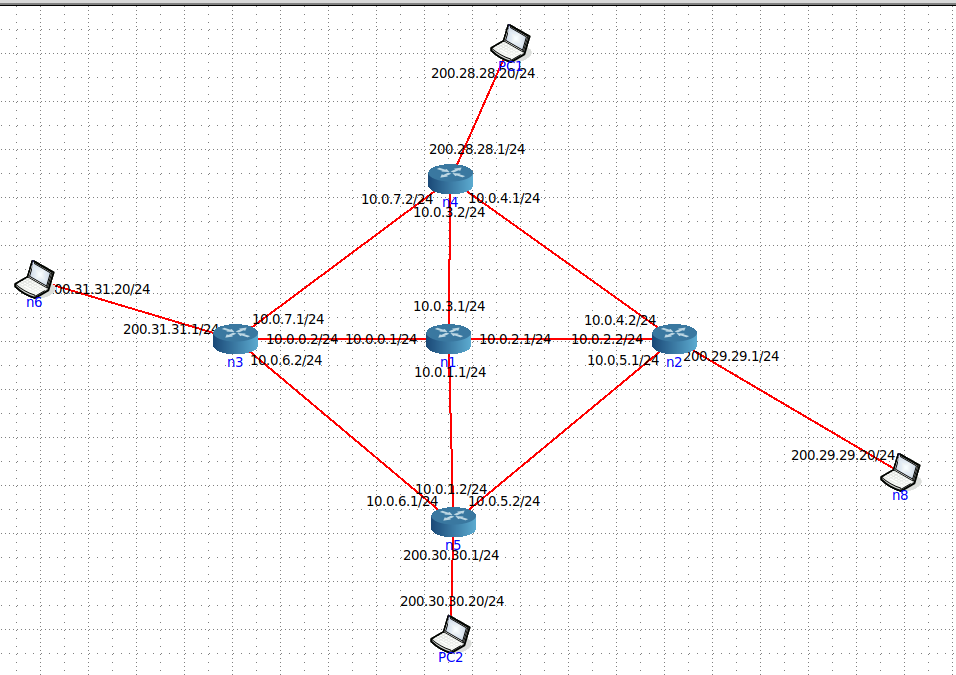
\includegraphics[width=1\textwidth]{images/rede.png}
    \caption{\label{fig:pacote}Implementação da topologia apresentada no CORE}
\end{figure}

\subsubsection{Numa shell do PC1, execute o comando traceroute para o endereço IP do PC2. Execute-o com a opção –I e depois sem esta opção. Registe e analise o tráfego enviado e recebido pelo PC1 decorrente do traceroute, em ambos os casos. Comente as diferenças observadas.}

\begin{figure}[h]
    \centering
    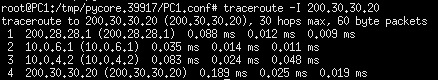
\includegraphics[width=1\linewidth]{images/traceroute-finI.png}
    \caption{Resultado do \textit{traceroute} com a flag -I}
    \label{fig:enter-label}
\end{figure}

\begin{figure}[h]
    \centering
    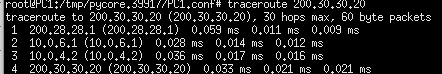
\includegraphics[width=1\linewidth]{images/traceroute-fin.png}
    \caption{Resultado do \textit{traceroute} sem a flag -I}
    \label{fig:enter-label}
\end{figure}

Ao executar o comando \texttt{traceroute} no PC1 para o endereço IP do PC2, foram obtidos os seguintes resultados:

\begin{verbatim}
root@PC1:/tmp/pycore.39917/PC1, conf# traceroute -I 200.30.30.20
traceroute to 200.30.30.20 (200.30.30.20), 30 hops max, 60 byte packets
1 200.28.28.1 (200.28.28.1) 0.088 ms 0.012 ms 0.009 ms
2 10.0.6.1 (10.0.6.1) 0.035 ms 0.014 ms 0.011 ms
3 10.0.4.2 (10.0.4.2) 0.083 ms
0.024 ms
0.048 ms
4 200.30.30.20 (200.30.30.20)
0.189 ms
0.025 ms 0.019 ms

root@PC1:/tmp/pycore.39917/PC1.conf# traceroute 200.30.30.20
traceroute to 200.30.30.20 (200.30.30.20), 30 hops max, 60 byte packets
1 200.28.28.1 (200.28.28.1) 0.059 ms 0.011 ms 0.009 ms
2 10.0.6.1 (10.0.6.1) 0.028 ms 0.014 ms 0.012 ms
3 10.0.4.2 (10.0.4.2) 0.036 ms
4 200.30.30.20 (200.30.30.20)
0.017 ms 0.033 ms
0.016 ms. 0.021 ms 0.021 ms
\end{verbatim}

Observa-se que, ao utilizar a opção \texttt{-I}, o comando \texttt{traceroute} utiliza o protocolo ICMP Echo Request, enquanto sem essa opção, ele utiliza UDP. Ambos os comandos revelam caminhos semelhantes, mas com diferenças nos tempos de resposta, o que é esperado ao usar diferentes protocolos (ICMP vs. UDP).


\subsubsection{Qual deve ser o valor inicial mínimo do campo TTL para alcançar o PC2? Verifique na prática que a sua resposta está correta.}

O comando \texttt{traceroute} foi executado com sucesso, e os resultados mostram os pacotes enviados e as respostas recebidas. Para determinar o valor inicial mínimo do campo TTL para alcançar o PC2, analisaremos os resultados.

A partir da saída fornecida:

\begin{figure}[h]
    \centering
    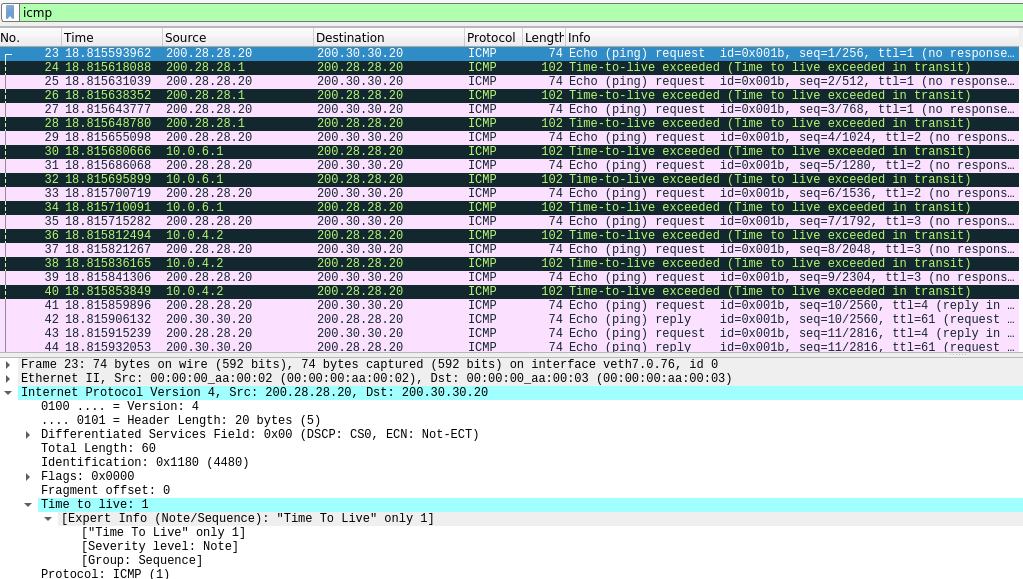
\includegraphics[width=0.8\linewidth]{images/ttlminnice.png}
    \caption{TTL Mínimo}
    \label{fig:enter-label}
\end{figure}

\begin{verbatim}
3   2.743738291   200.28.28.20   200.31.31.20   ICMP   74   Echo (ping) request
                                                       id=0x001e, seq=1/256, ttl=1 (no response found!)
\end{verbatim}

O primeiro pacote foi enviado com TTL igual a 1, e a resposta mostra "Time-to-live exceeded (Time to live exceeded in transit)". Isso indica que o pacote atingiu o limite de TTL ao chegar ao destino. Portanto, o valor inicial mínimo do campo TTL para alcançar o PC2 é 1.

Este resultado é consistente com o esperado, pois há 4 saltos entre o PC1 e o PC2, e começar com TTL = 1 permite que o pacote atinja o destino com sucesso.


\subsubsection{Com base na informação obtida pelo traceroute –I, responda:}

\begin{figure}[h]
    \centering
    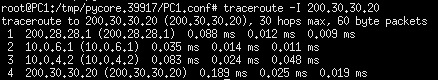
\includegraphics[width=0.8\linewidth]{images/traceroute-finI.png}
    \caption{Resultado do comando \textit{traceroute} com a flag -I}
    \label{fig:enter-label}
\end{figure}

\begin{enumerate}    
    \item \textbf{Quais são os routers percorridos pelos pedidos gerados pelo \texttt{traceroute}?}

    \textbf{i.} Os routers percorridos pelos pedidos gerados pelo \texttt{traceroute} são:
    
    \begin{itemize}
        \item Router N2 com o IP 10.0.6.1
        \item Router N5 com o IP 10.0.4.2
    \end{itemize}

    \item \textbf{As rotas seguidas pelos pacotes de pedido e resposta são iguais, mas em sentidos contrários? Justifique.}

    A rota seguida pelos pacotes é:
    \begin{itemize}
        \item PC1 (200.28.28.1) $\rightarrow$ Router N2 (10.0.6.1) $\rightarrow$ Router N5 (10.0.4.2) $\rightarrow$ PC2 (200.30.30.20)
    \end{itemize}

    A rota seguida pelos pacotes de pedido e resposta é a mesma, mas em sentidos contrários. Isso é evidente ao comparar os IPs de origem e destino nos resultados fornecidos. O pacote vai do PC1 ao PC2 e, em seguida, a resposta vai do PC2 ao PC1, indicando a mesma rota, mas em direções opostas.
\end{enumerate}

\subsubsection{Calcule o valor médio do tempo de ida-e-volta (Round-Trip Time) obtido, indicando de forma clara como obteve esse valor. Para melhorar a média, use seis probe packets , usando para tal a opção -q.}

\begin{align*}
\text{Média RTT}_1 &= \frac{0.088 + 0.012 + 0.009}{3} \\
\text{Média RTT}_2 &= \frac{0.035 + 0.014 + 0.011}{3} \\
\text{Média RTT}_3 &= \frac{0.083 + 0.024 + 0.048}{3} \\
\text{Média RTT Geral} &= \frac{\text{Média RTT}_1 + \text{Média RTT}_2 + \text{Média RTT}_3}{3}
\end{align*}

\subsection{Use agora o traceroute na sua máquina nativa. (N.B.: o tracert disponibilizado no Windows não permite mudar o tamanho das mensagens a enviar. Porém, no Linux/Mac, o traceroute permite indicar o tamanho do pacote ICMP através da linha de comando, a seguir ao host de destino - ver man traceroute. Por exemplo, traceroute -I router-di.uminho.pt 512). Usando o Wireshark, capture o tráfego gerado pelo seginte comando: traceroute -I marco.uminho.pt (Linux/Mac); tracert marco.uminho.pt (Windows). Pare a captura. Com base no tráfego capturado, identifique os pedidos ICMP Echo Request e o conjunto de mensagens devolvidas como resposta. Selecione a primeira mensagem ICMP capturada e centre a análise no nível protocolar IP (expanda o tab correspondente na janela de detalhe do Wireshark). Através da análise do cabeçalho IP diga:}

\begin{figure}[h]
    \centering
    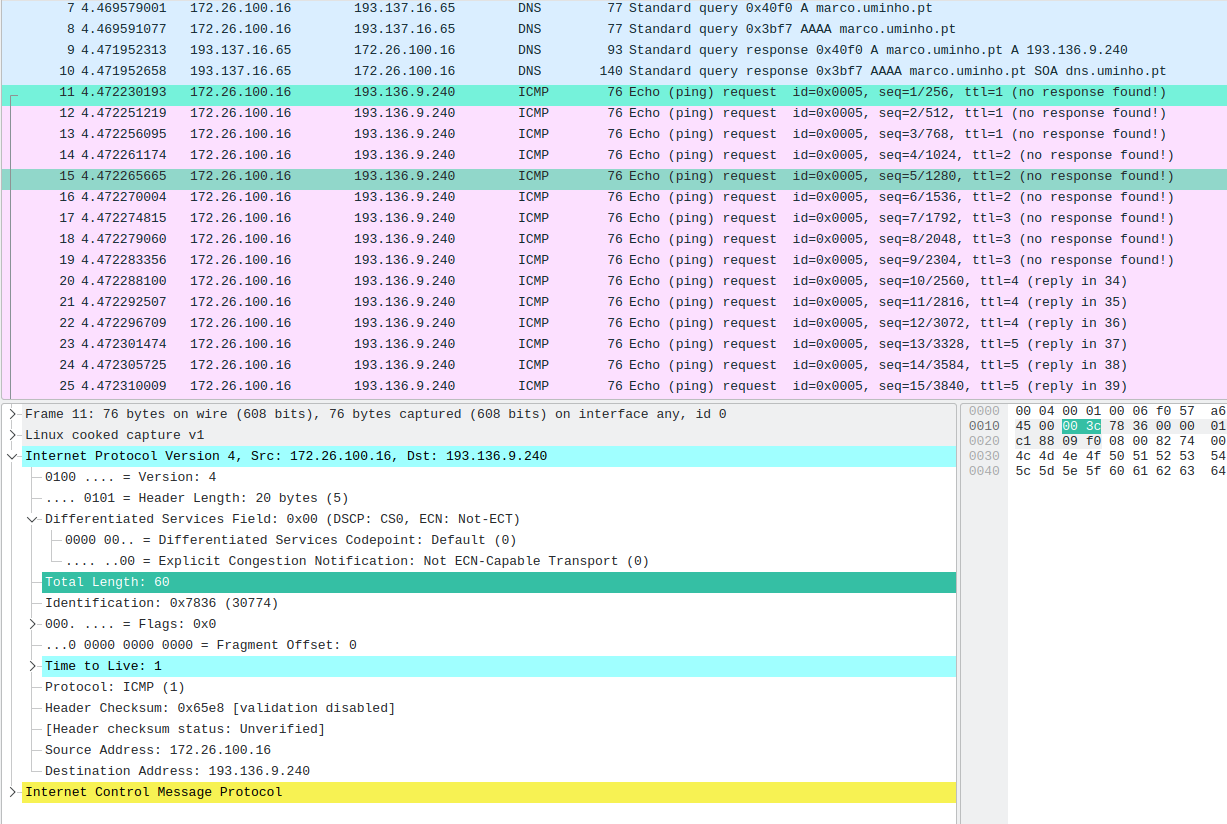
\includegraphics[width=1\textwidth]{images/PacoteQuestao2.png}
    \caption{\label{fig:pacote}Pacote no wireshark}
\end{figure}

\subsubsection{Qual é o endereço IP da interface ativa do seu computador?}

O endereço IP da interface ativa do computador será o Source Address, que neste caso é \textbf{172.26.100.16}.

\subsubsection{Qual é o valor do campo Protocolo? O que identifica?}

O valor é ICMP (1). O Protocolo ICMP é utilizado para vários diagnósticos de rede e reports em erros de funções, o significado dos valores varia de acordo com o tipo específico no campo Protocolo.

\subsubsection{Quantos bytes tem o cabeçalho IPv4? Porque razão essa informação está
presente no cabeçalho IP, ao contrário do cabeçalho MAC?}

O cabeçalho IPv4 possui 20 bytes, indicado em \textit{\textbf{Header Length}}. Essa informação está presente no cabeçalho IP pois atua num nível mais alto na pilha de protocolos OSI model. O protocolo IPv4 atua no nível 3, que é a camada de rede, já o cabeçalho MAC está presente no nível 2, que é camada de data link.

\subsubsection{Quantos bytes tem o campo de dados (payload) do datagrama? Como se
calcula o tamanho do payload?}

O payload possui 40 bytes. Tamanho do Payload = Tamanho total do IPv4 - Tamanho do cabeçalho IPv4 

\subsubsection{O datagrama IP foi fragmentado? Justifique.}

Não. Podemos observar se um datagrama IP foi fragmentado analisando as suas flags. Nesse caso, as flags são \textit{\textbf{000}}, que significa que não foram colocadas (not set), que é a mesma coisa de não estar fragmentado. Além disso, podemos analisar o Fragment Offset, que está todo zerado, isso signifca que ele seria o primeiro fragmento do datagrama fragmentado e, como as flags são todas 0's, não existem mais fragmentos.

\subsubsection{Ordene os pacotes capturados de acordo com o endereço IP fonte, e
analise a sequência de tráfego ICMP gerado a partir do endereço IP
atribuído à interface da sua máquina. Para a sequência de mensagens
ICMP enviadas pelo seu computador, indique que campos do cabeçalho
IP variam de pacote para pacote.}

Os campos do cabeçalho IP que variam de pacote para pacote são: \textbf{Identification} e \textbf{Header Checksum}

\subsubsection{Qual é o valor do campo TTL? Esse valor permanece constante
para todas as mensagens de resposta ICMP TTL exceeded
enviados ao seu host? Porquê?}

O valor do campo TTL é 254. Não permanece constante para todas as mensagens de resposta ICMP TTL exceeded. O TTL é decrementado em 1 a cada salto de roteador. Quando o TTL atinge zero, o roteador descarta o pacote e envia uma mensagem ICMP "TTL Exceeded" de volta ao remetente. O valor do TTL pode variar de pacote para pacote, dependendo do número de saltos que cada pacote faz na rede.

\subsubsection{Porque razão as mensagens de resposta ICMP TTL Exceeded são
sempre enviadas na origem com um valor TTL relativamente
alto?}

Com um valor TTL alto, o ping durará mais tempo antes de expirar, há mais flexibilidade para o pacote atravessar uma variedade de redes antes de atingir seu destino.

\subsubsection{Comente a rota obtida, destacando os aspetos que considera mais
significativos.}

O pacote atravessou vários países antes de chegar em Portugal, primeiro saiu dos EUA e chegou na Europa pelo Reino Unido, Alemanha e Holanda, somente depois foi para Portugal. Foram 21 saltos até chegar no servidor da Universidade do Minho, em Lisboa, e demorou em torno de 1 segundo para chegar ao destino final.

\subsubsection{Analisando os tempos de resposta e as perdas de pacotes, diga,
justificando, se nessa rota há algum nó com um possível
congestão de tráfego e/ou problema de outra natureza.}

Quando uma maior distância é percorrida pelo pacote, o tempo de resposta aumenta, por exemplo, quando o pacote vem dos EUA para a Europa pelo oceano atlântico é, em média, 100ms, ao contrário quando os pacotes são de curta distância, que possui um response time de 2ms dentro os EUA. Não houve perda de pacotes. Porém, podemos observar um outro problema de outra natureza: Os pacotes chegaram na Europa por Londres, ao invés de chegarem diretamente em Portugal. Isso acontece por não haver ligação direta entre a América do Norte e Portugal por cabos subsubaquáticos no oceano atlântico.

\subsection{Analise da fragmentação de pacotes IP}

Foi capturado o tráfego gerado pelo comando: ping -s 6328 marco.uminho.pt

\begin{figure}[h]
    \centering
    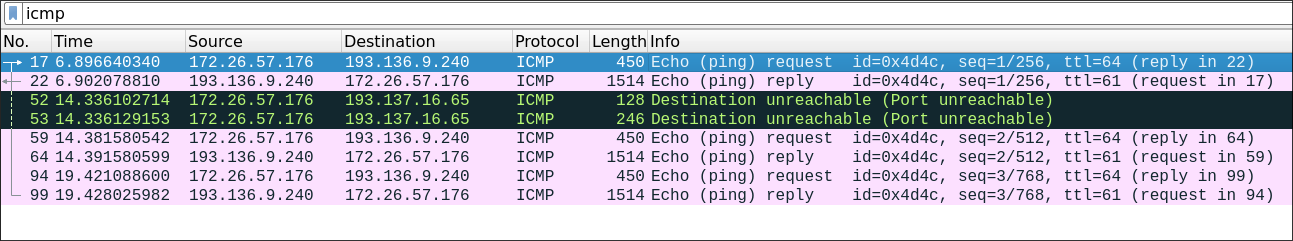
\includegraphics[width=0.8\textwidth]{images/ping.png}
    \caption{\label{fig:ping}Ping}
\end{figure}

\subsubsection{Localize a primeira mensagem ICMP.}
\subsubsection{Porque é que houve necessidade
de fragmentar o pacote inicial?}
\begin{figure}[h]
    \centering
    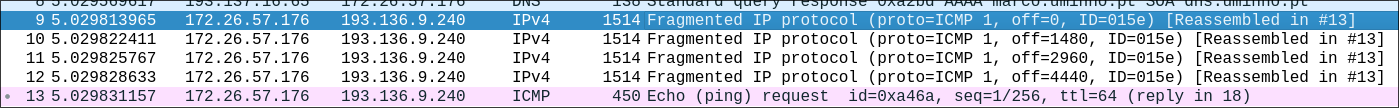
\includegraphics[width=0.8\textwidth]{images/fragment.png}
    \caption{\label{fig:fragment}Fragment}
\end{figure}

A necessidade surge de o facto de o tamanho do pacote ser superior ao MTU da rede, ou seja, não cabe num único pacote. O MTU da rede é de 1500 bytes, e o tamanho do pacote é de 6328 bytes, logo é necessário fragmentar o pacote.

\subsubsection{Em que equipamento da rede ocorreu essa fragmentação?}

A fragmentacao ocorreu no computador que enviou o pacote. 

\subsubsection{Imprima o primeiro fragmento do datagrama IP.}
\subsubsection{Que informação no cabeçalho indica que o datagrama foi fragmentado?}

A opcao MF, que indica que o pacote foi fragmentado, pode ser observada no wireshark, dentro do campo Flags, no cabeçalho IP.

\begin{figure}[h]
    \centering
    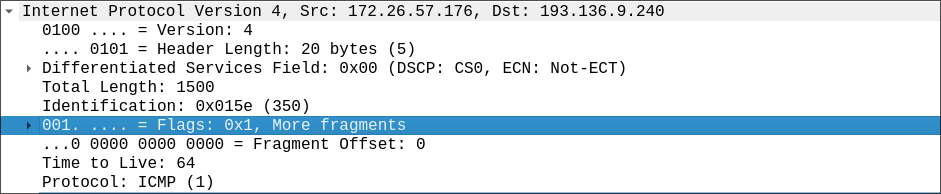
\includegraphics[width=0.8\textwidth]{images/mf.png}
    \caption{\label{fig:more_fragments}More Fragments}
\end{figure}

\subsubsection{Que informação
no cabeçalho IP indica que se trata do primeiro fragmento?}

O campo Fragment Offset indica que se trata do primeiro fragmento, uma vez que o seu valor é 0.

\subsubsection{Qual é o tamanho deste fragmento?}

O tamanho do fragmento é de 1500 bytes, tal como indica o campo Total Length.

\subsubsection{Imprima o segundo fragmento do datagrama IP original. Que informação
do cabeçalho IP indica que não se trata do primeiro fragmento? Há mais
fragmentos? O que nos permite afirmar isso?}

\begin{figure}[h]
    \centering
    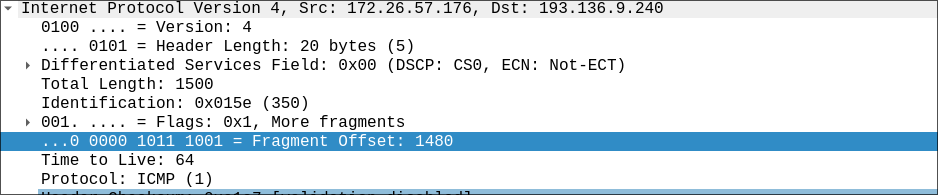
\includegraphics[width=0.8\textwidth]{images/mf_offset.png}
    \caption{\label{fig:more_fragments_offset}More Fragments Com Offset}
\end{figure}

O campo Fragment Offset indica que não se trata do primeiro fragmento, uma vez que o seu valor é 1480. O campo MF indica que há mais fragmentos, uma vez que o seu valor é 1.
Logo basta que: Fragment Offset != 0 $\wedge$ MF == 1 para sabermos que não se trata do primeiro fragmento.

\subsubsection{Indique os campos que mudam no cabeçalho IP entre os diferentes
fragmentos, e explique a forma como essa informação permite
reconstruir o datagrama original.}

Os campos que mudam sao:
\begin{itemize}
    \item Flag More Fragments (MF)
    \item Fragment Offset
    \item Total Length
\end{itemize}
Os campos que permitem reconstruir o datagrama original, sao o Fragment Offset, e a flag MF, pois estes permitem saber a ordem exata dos fragmentos, de forma a reconstruir tal e qual como antes de ser fragmentado.

\subsubsection{Como se deteta o último fragmento correspondente ao datagrama
original? Estabeleça um filtro no Wireshark que permita listar o último
fragmento do primeiro datagrama IP segmentado.}

ip.flags.mf == 0

\subsubsection{Identifique o equipamento onde o datagrama IP original é reconstruído a
partir dos fragmentos. A reconstrução poderia ter ocorrido noutro
equipamento diferente do identificado? Porquê?}

O equipamento onde o datagrama IP original é reconstruído é o servidor de IP: 193.136.9.240, ou seja, o servidor de marco.uminho.pt. A reconstrução poderia ter ocorrido noutro equipamento desde que a MTU fosse superior a MTU da ligacao anterior, ou seja maior que 1500 bytes, e que o equipamento tivesse a capacidade de reconstruir o datagrama original.

\subsubsection{Por que razão apenas o primeiro fragmento de cada pacote é identificado
como sendo um pacote ICMP?}

Apenas o primeiro fragmento de cada pacote é identificado como sendo um pacote ICMP, pois o conceito de ICMP tem por base os cabecalhos IP, e o conceito de fragmentacao de datagramas IP e relativo ao cabecalho IP.

\subsubsection{Determine o valor máximo de SIZE sem que ocorra
fragmentação do pacote? Justifique o valor obtido, relacionando-o com o
MTU (Maximum Transmission Unit) da rede.}

Apos observar o output do comando ping no linux:
\begin{figure}[h]
    \centering
    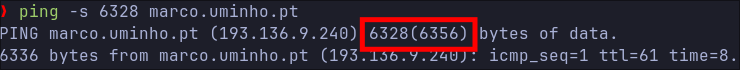
\includegraphics[width=0.8\textwidth]{images/ping_cmd.png}
    \caption{\label{fig:ping_cmd}Comando Ping no Linux}
\end{figure}
Reparei que houve um acrescimo de 28 bytes na informacao enviada, para acomodar todos os cabecalhos essenciais na trasnmissao do pacote.
Logo o valor maximo de SIZE sem que ocorra fragmentacao do pacote e de 1472 bytes, pois 1472 + 28 = 1500 bytes, que e o MTU da rede.

\section{Parte 2}
\subsection{Endereçamento e Encaminhamento IP}
\subsubsection{Atribua um conjunto de endereços IP válidos (públicos) aos diversos sistemas da
GEO, devendo o seu nº de grupo estar presente em pelo menos um octeto da
componente de rede. Use máscaras (prefixos) de rede que respeitem a divisão
clássica de endereçamento por classes (ver a tabela em anexo).}

\subsubsection{Apresente uma imagem com o esquema de endereçamento usado na
rede da GEO.}

\begin{figure}[h]
    \centering
    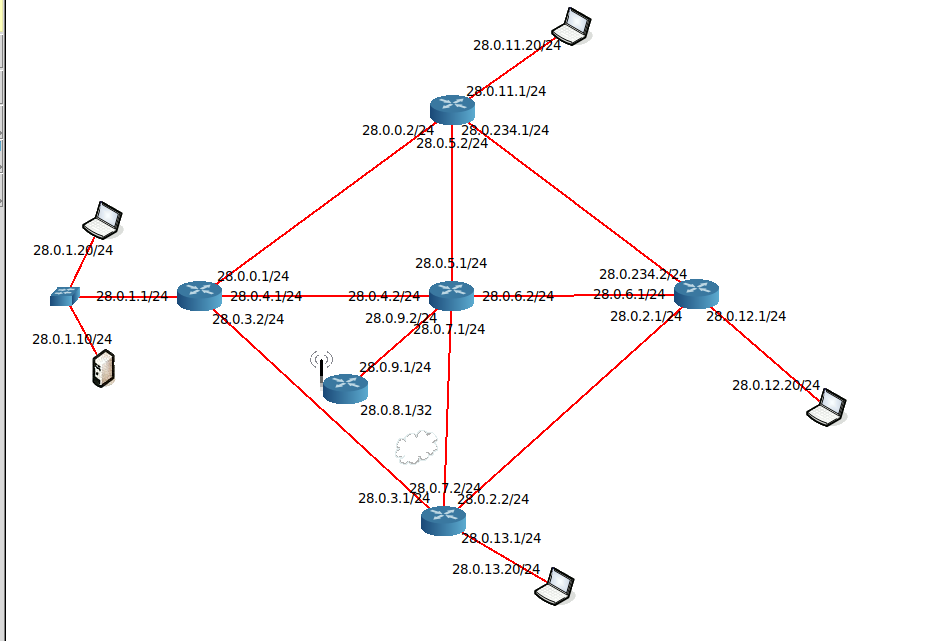
\includegraphics[width=1\textwidth]{images/aularedes.png}
    \caption{\label{fig:pacote}Diagrama da rede}
\end{figure}

\subsubsection{Escolha um endereço IP atribuida a uma interface de rede e, recorrendo
ao operador lógico AND, explique como a máscara de rede permite
identificar as suas componentes de rede e de host?}

Pegando o endereço IP 28.0.234.34/24 e a máscara de rede 255.255.255.0, temos:

\begin{figure}[h]
    \centering
    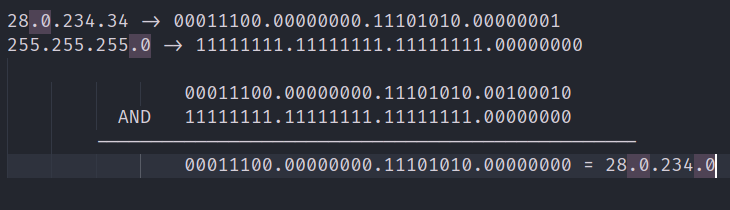
\includegraphics[width=1\textwidth]{images/ANDlogic.png}
    \caption{\label{fig:pacote}AND lógico}
\end{figure}

A resposta final do AND lógico será 00011100.00000000.11101010.00000000, que é o equivalente a 28.0.234.0 em decimal. Este valor será a componente de rede do IP com a máscara 255.255.255.0 (/24). Podemos concluir que a máscara ao efetuar o AND lógico irá zerar os valores que constituem os hosts e os restantes valores será a rede.

\subsubsection{Faria sentido o CORE atribuir um endereço IP aos switches? Justifique.}

Não, os switches são aparelhos layer 2. Apesar de existirem switches layer 3 que administram o destino dos pacotes através de endereços IP, a maior parte dos switches são layer 2, consequentemente, o destino dos dados será feito com MAC Adresses.

\subsection{Para o router RA e o servidor do departamento A, execute o comando netstat –rn para consultar a tabela de encaminhamento unicast (IPv4). Inclua no seu relatório as tabelas de encaminhamento obtidas. Se necessário, consulte o manual (man route) para esclarecer os detalhes sobre as tabelas de encaminhamento.}

\begin{figure} [h]
    \centering
    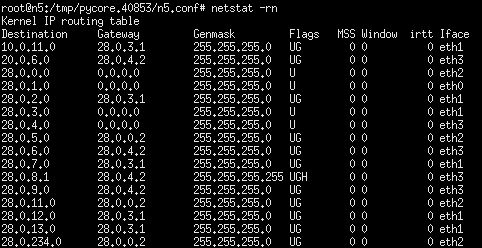
\includegraphics[width=0.75\linewidth]{images/ra.png}
    \caption{Resultado do comando \textit{netstat –rn}
para consultar a tabela de encaminhamento unicast (IPv4) do router do departamento A.}
    \label{fig:enter-label}
\end{figure}

\begin{figure} [h]
    \centering
    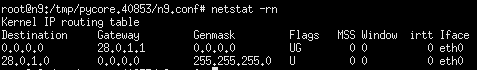
\includegraphics[width=0.75\linewidth]{images/servera.png}
    \caption{execute o comando netstat –rn
para consultar a tabela de encaminhamento unicast (Resultado do comando \textit{netstat –rn}
para consultar a tabela de encaminhamento unicast (IPv4) do servidor do departamento A.}
    \label{fig:enter-label}
\end{figure}

\subsubsection{Considere que ao router RA chega um pacote IP proveniente do host dum outro departamento (à sua escolha) e destinado ao servidor. Descreva detalhadamente como esse router encaminha o pacote usando a sua tabela de encaminhamento.}

Suponha que um pacote IP chega ao Router RA proveniente de um host de outro departamento com destino ao servidor (por exemplo, IP de origem: 28.0.x.x, IP de destino: 28.0.1.10). O encaminhamento seria feito de acordo com a tabela do Router RA, passando por cada rota até alcançar a rede do servidor.

\subsubsection{Encaminhamento de Pacotes para 28.0.1.10 no Router do Departamento A}

Quando o servidor responde ao host de outro departamento, ele consulta sua tabela de encaminhamento. A rota para 0.0.0.0, que representa qualquer destino fora das redes locais, apontará para o gateway 28.0.1.1, que é o Router RA. O Router RA, por sua vez, encaminhará o pacote para o destino correto com base na sua tabela.


\subsection{Diga, justificando, se na rede está a ser usado encaminhamento estático ou
dinâmico (e.g. baseado no protocolo OSPF - Open Shortest Path First). (Sugestão:
analise os processos que estão a correr em cada sistema (hosts, routers) usando,
por exemplo, o comando ps -ax).}

\begin{figure}[h]
    \centering
    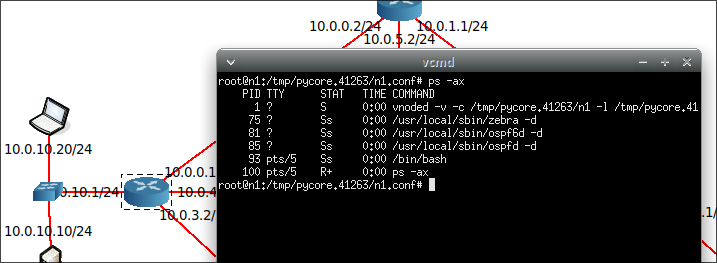
\includegraphics[width=0.8\textwidth]{images/ospf.png}
    \caption{\label{fig:ospf}OSPF no router}
\end{figure}

Conforme a figura acima demonstra, o router esta a usar o protocolo OSPF, logo esta a usar encaminhamento dinamico, pois nao foi necessario especificar as rotas manualmente, e o protocolo ficou responsavel por isso.

\subsection{A rota das mensagens ICMP echo reply é a mesma, mas em
sentido inverso, da rota das mensagens ICMP echo request
trocadas entre esse PC e o servidor? Justifique. (Sugestão: trace a
rota do servidor para o PC selecionado, e vice-versa).}

Sim. Ao fazermos traceroute de um PC para o servidor, obtemos um caminho semelhante à rota do servidor para o PC, mas em sentido contrário, como podemos observar na imagem.

\begin{figure}[h]
    \centering
    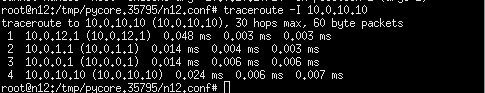
\includegraphics[width=1\textwidth]{images/pctoserver.png}
    \caption{\label{fig:pacote}Rota do traceroute de um PC para o servidor}
\end{figure}

\begin{figure}[h]
    \centering
    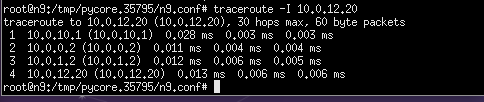
\includegraphics[width=1\textwidth]{images/servertopc.png}
    \caption{\label{fig:pacote}Rota do traceroute do servidor para um PC}
\end{figure}

\subsubsection{Em caso afirmativo à resposta anterior, altere as tabelas de
encaminhamento dos sistemas de forma que as rotas dos pedidos
e das respostas sejam diferentes. Em caso negativo, altere as
tabelas de encaminhamento para que as rotas dos pedidos e das
respostas sejam iguais. (Use os comandos route add e route del
para alterar as tabelas de encaminhamento – consulte o man
route). Apresente as tabelas de encaminhamento alteradas e os
comandos usados para tal. Prove com o traceroute que se
alcançaram as rotas pretendidas.}

Utilizando os comandos: \textbf{route del -net 10.0.5.0 netmask 255.255.255.0 gw 10.0.0.2} e  \textbf{route add -net 10.0.5.0 netmask 255.255.255.0 gw 10.0.4.2} excluímos a hipótese de o pedido ICMP passar por 10.0.0.2 e mudar a sua rota para 10.0.4.2. Teremos que fazer isso para todos os Gateways que possuem 10.0.0.2 de forma a evitar esse caminho.

\begin{figure}[h]
    \centering
    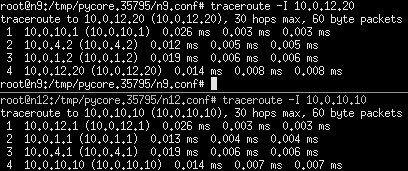
\includegraphics[width=1\textwidth]{images/routes.png}
    \caption{\label{fig:pacote}Ambos os traceroutes invertidos e agora com um caminho do pedido ICMP diferente do anterior}
\end{figure}

\subsection{Por razões administrativas, admita que a rota por defeito (0.0.0.0 ou default) foi retirada definitivamente da tabela de encaminhamento do servidor do departamento A. Use o comando route del para o efeito.}

\begin{enumerate}
    \item \textbf{Que implicações tem esta medida para os utilizadores que acedem ao servidor? Justifique.}

    \begin{itemize}
        \item A remoção da rota padrão na tabela de encaminhamento do servidor do departamento A significa que o servidor não tem uma rota predefinida para enviar pacotes para destinos fora das redes diretamente conectadas a ele.
        \item Os utilizadores que tentarem aceder a recursos externos (fora das redes locais) a partir do servidor enfrentarão a incapacidade de alcançar esses destinos, resultando em falhas de conectividade.
    \end{itemize}

    \item \textbf{Adicione as rotas estáticas necessárias para restaurar a conectividade ao servidor, por forma a contornar a restrição imposta na alínea anterior e dar acesso ao servidor apenas aos utilizadores internos da GEO, mas não aos utentes externos (através do router wireless RISP).}

    \begin{enumerate}
        \item \textbf{Apresente os comandos usados e as tabelas de encaminhamento alteradas. Com o comando ping, teste a nova política de encaminhamento garantindo que o servidor está acessível apenas para os utilizadores internos da GEO, mas não aos externos}


        Para contornar a restrição e restaurar a conectividade ao servidor, devem ser adicionadas rotas estáticas para os destinos desejados. Supondo que se deseja permitir apenas o acesso aos utilizadores internos da GEO e não aos utentes externos (através do router wireless RISP), as rotas estáticas serão configuradas de acordo. Exemplo de comandos (considerando que o endereço IP do RISP seja 28.0.0.2):
        
        \begin{verbatim}
route add -net 0.0.0.0 netmask 0.0.0.0 gw 28.0.0.2 dev eth1
\end{verbatim}
    
        \item \textbf{Teste com Comando Ping:}

        Após a adição das rotas estáticas, é essencial testar a nova política de encaminhamento. Usamos o comando ping para verificar se o servidor está acessível apenas para os utilizadores internos da GEO. 
        Exemplo de comando ping (assumindo o IP 28.0.1.10 para o servidor):
        
        \begin{verbatim}
            ping -c 4 28.0.1.10
        \end{verbatim}
    
        É necessário verificar que o servidor responde aos utilizadores internos, mas não responde aos utentes externos através do router wireless RISP.
    \end{enumerate}
\end{enumerate}

\subsubsection{Apague na tabela de encaminhamento do router de cada departamento e do
router central a entrada respeitante à rede da interface wireless do router RISP.
Confirme que os sistemas da GEO deixaram de ter acesso à interface wireless do
router RISP. Usando apenas rotas por defeito, altere as tabelas de
encaminhamento desses routers de forma a tornar novamente acessível o acesso
à Internet através da interface wireless do router RISP.}

Apos apagar a entrada respeitante a rede da interface wireless do router RISP, os sistemas da GEO deixaram de ter acesso a interface wireless do router RISP, pois nao sabem para onde encaminhar os pacotes.
\begin{figure}[h]
    \centering
    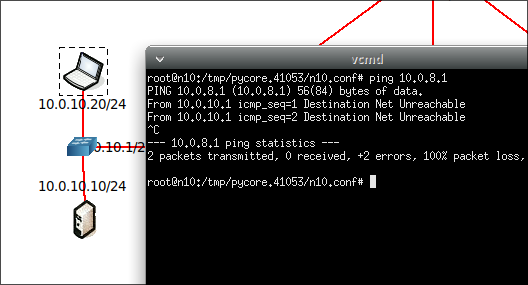
\includegraphics[width=0.8\textwidth]{images/before-route.png}
    \caption{\label{fig:before_route}Antes de routing manual}
\end{figure}

Para retormar o acesso a interface wireless do router RISP, foi necessario adicionar 2 rotas manualmente.
\begin{figure}[h]
    \centering
    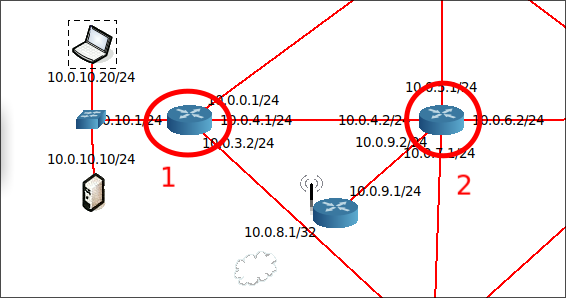
\includegraphics[width=0.8\textwidth]{images/route.png}
    \caption{\label{fig:route}Routing manual}
\end{figure}

\begin{itemize}
    \item No router 1 foi executado o comando: ip route add default via 10.0.4.2
    \item No router 2 foi executado o comando: ip route add default via 10.0.9.1
\end{itemize}

Mas de forma a retornar a conexao de cada departamento a internet, foi necessario adicionar uma rota por defeito no router de cada departamento em direcao ao router central, seguindo o mesmo esquema: ip route add default via "ip do router central".

Apos testar, todos os departamentos conseguiram aceder a internet.

\subsection{Definição de Sub-redes}
\subsubsection{Apresente uma imagem que mostre claramente o esquema de
endereçamento de subredes adotado. Deve justificar as opções tomadas.}

Tem em conta que existem 4 departamentos, apenas seriam necessarios 2 bits para representar as 4 subredes, mas como o enunciado pede que seja reservada pelo menos uma rede para uso futuro, foram reservados 3 bits para representar as subredes, ou seja, 8 subredes.

Logo as subredes seguem o seguinte formato de endereçamento, tendo por base o endereco 10.0.10.xx/24:
\begin{itemize}
    \item Subrede 1 - 10.0.10.0/27 - sendo .0 o valor do ultimo octeto, com o bit \[2^7 = 0 \land 2^6 = 0 \land 2^5 = 0\]
    \item Subrede 2 - 10.0.10.64/27 - sendo .64 o valor do ultimo octeto, com o bit \[2^7 = 0 \land 2^6 = 1 \land 2^5 = 0\]
    \item Subrede 3 - 10.0.10.128/27 - sendo .128 o valor do ultimo octeto, com o bit \[2^7 = 1 \land 2^6 = 0 \land 2^5 = 0\]
    \item Subrede 4 - 10.0.10.192/27 - sendo .192 o valor do ultimo octeto, com o bit \[2^7 = 1 \land 2^6 = 1 \land 2^5 = 0\]
\end{itemize}

\begin{figure}[h]
    \centering
    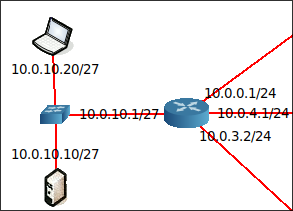
\includegraphics[width=0.8\textwidth]{images/subnetting.png}
    \caption{\label{fig:subnetting}Subnetting}
\end{figure}

\subsubsection{Qual a máscara de rede que usou? Quantos hosts IP
pode interligar no máximo em cada departamento? Quantos endereços
de sub-rede ficam disponíveis para uso futuro? Justifique.}

A mascara de rede usada foi 255.255.255.192, em formato CIDR /27 pois foram reservados 3 bits para representar as subredes, dos ja reservados 24 bits para representar a rede principal.
Sobram-nos 5 bits para representar os hosts, logo temos 32 enderecos disponiveis para hosts, mas como o endereco de rede e o endereco de broadcast nao podem ser usados, ficam disponiveis 30 enderecos para hosts.
A nivel das subredes, ficam disponiveis 4 subredes para uso futuro, pois das 8 subredes possiveis, apenas foram usadas 4.

\subsubsection{Garanta e verifique que a conectividade IP entre os vários
departamentos é mantida. Explique como procedeu.}

Para verificar a conectividade, foi feito ping de cada departamento para cada departamento, e todos os pings foram bem sucedidos.

\section{Conclusao}

Neste relatório, adquiri conhecimento e habilidades significativas no uso de diversos utilitários essenciais. Entre eles, destaco o traceroute, o ping, e o ip route, que se revelaram fundamentais para explorar a estrutura da rede. A aplicação dessas ferramentas não apenas aprimorou a minha compreensão sobre subnetting, como também contribuiu para uma percepção mais ampla sobre como dimensionar uma rede de forma eficiente.

Além disso, a experiência com esses utilitários proporcionou um entendimento mais profundo sobre a fragmentação de pacotes em relação à Maximum Transmission Unit (MTU) da rede. Essa compreensão é crucial para otimizar a transmissão de dados e garantir um desempenho eficaz da rede.

Destaco ainda que o uso do traceroute não apenas foi valioso para identificar caminhos de comunicação, como também ampliou a minha consciência sobre a performance da comunicação na internet.

\end{document}
